\documentclass[11pt]{article}

\usepackage[margin=1in]{geometry}
\usepackage{setspace}
\onehalfspacing
\usepackage{graphicx}
\graphicspath{report_images/}
\usepackage{appendix}
\usepackage{listings}
\usepackage{float}
\usepackage{multirow}
\usepackage{amsthm}
% The next three lines make the table and figure numbers also include section number
\usepackage{chngcntr}
\counterwithin{table}{section}
\counterwithin{figure}{section}
% Needed to make titling page without a page number
\usepackage{titling}

% DOCUMENT INFORMATION =================================================
\font\titleFont=cmr12 at 11pt
\title {{\titleFont ECEN 429: Introduction to Digital Systems Design Laboratory \\ North Carolina Agricultural and Technical State University \\ Department of Electrical and Computer Engineering}} % Declare Title
\author{\titleFont Reporter: Nikiyah Beulah \\ \titleFont Partner: Chris Cannon} % Declare authors
\date{\titleFont April 5, 2018}
% ======================================================================

\begin{document}

\begin{titlingpage}
\maketitle
\begin{center}
	Lab 10
\end{center}
\end{titlingpage}

\section{Introduction}
This lab prompts us to implement a vending machine of our own design, within given specifications. Vending machines are an approachable implementation of finite state machines that can have varying levels of complexity, making them ideal for this lab. Our vending machine will use what we have learned about clocks, state machines, and inputs/outputs to make a real world device.

\section{Background, Design Solution, and Results}

\subsection{Problem 1 }

\subsubsection{Background}
This vending machine can dispense one of two items, gum or candy. Gum costs 15 cents and candy costs 20 cents. This machine does not provide change, which makes things easier for us because we need only know whether or not we exceeded the required amount, and not by how much.

\subsubsection{Design Solution}
This solution is a simple Moore state machine, as shown in Figure ~\ref{fig:lab10_state_diagram}. This Moore machine is designed with a state to dispense gum and a state to dispense candy. Any money input after the maximum values (20 cents) has been reached, is assumed to be automatically returned to the user, so not additional amount is recorded and no state progression takes place. We also included an "amount" output on the LEDs that would represent each of our possible states, with 0 cents as the least significant LED (on the right) and 20 cents as the most significant LED (on the left). The inputs for this implementation are summarized in Table ~\ref{tab:lab10_input_Ports} and Table ~\ref{tab:lab10_output_Ports}.

\begin{table}[H]
\begin{center}
\begin{tabular}{| l | l | l |}
	\hline
	Bit & Label & Port \\ \hline
	clk & Clock & W5 \\ \hline
	candy & Button Right & T17 \\ \hline
	gum & Button Left & W19 \\ \hline
	nickel & Button Top & T18 \\ \hline
	dime & Button Bottom & U17 \\ \hline
	reset & Button Center & U 18 \\ \hline
\end{tabular}
\caption{\label{tab:lab10_input_Ports}Input port assignments for  the vending machine.}
\end{center}
\end{table}

\begin{table}[H]
\begin{center}
\begin{tabular}{| l | l | l |}
	\hline
	Bit & Label & Port \\ \hline
	clk led & LED 15 & L1 \\ \hline
	amount 4 & LED 4 & W18 \\ \hline
	amount 3 & LED 3 & V19 \\ \hline
	amount 2 & LED 2 & U19 \\ \hline
	amount 1 & LED 1 & E19 \\ \hline
	amount 0 & LED 0 & U16 \\ \hline
\end{tabular}
\caption{\label{tab:lab10_output_Ports}Output port assignments for the vending machine.}
\end{center}
\end{table}

\begin{figure}
\begin{center}
	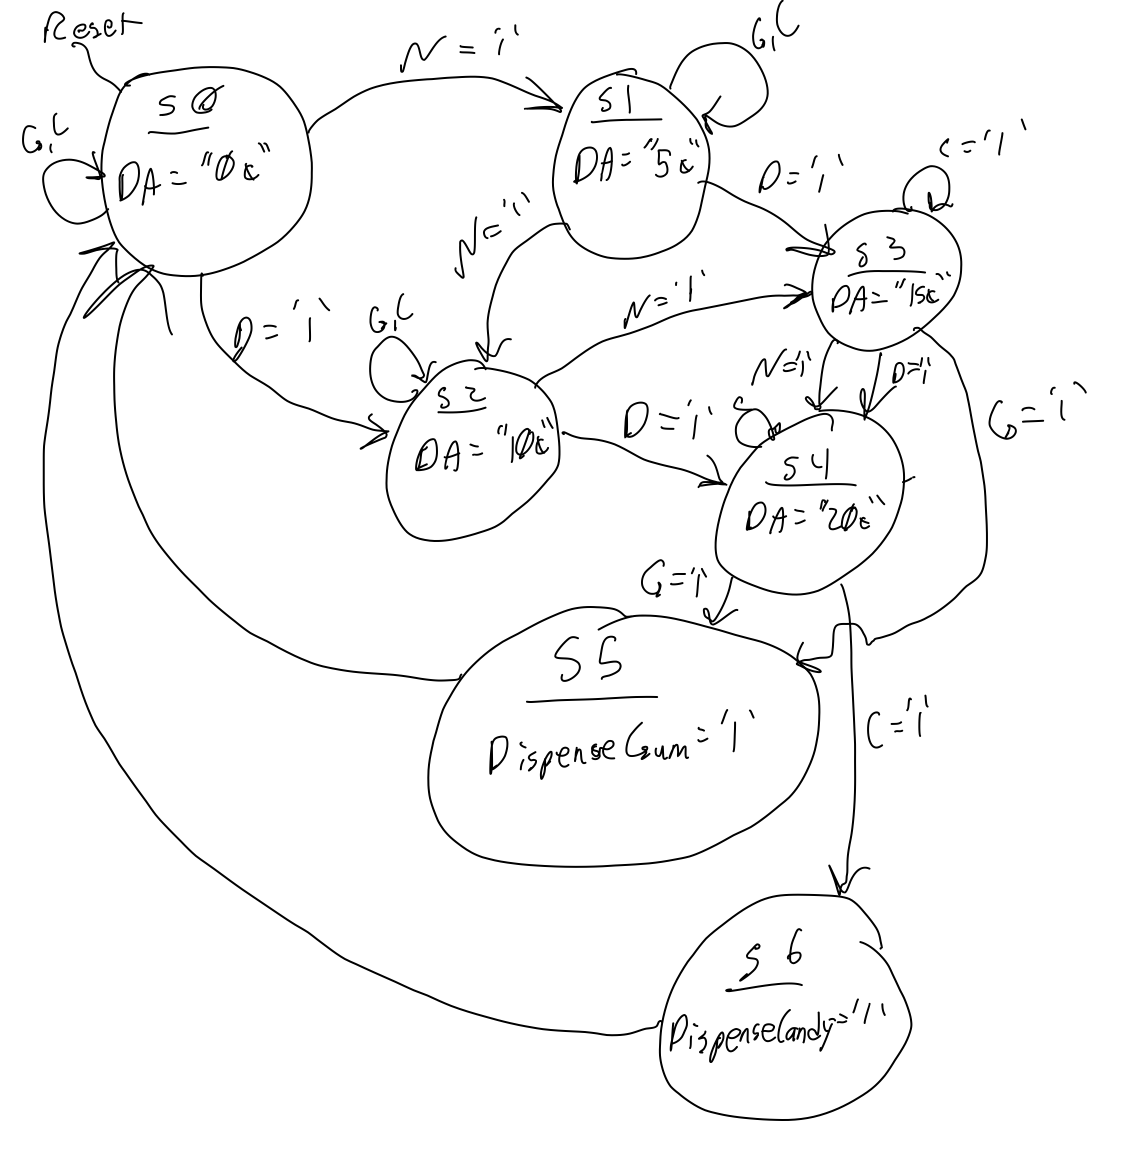
\includegraphics[width=0.5\textwidth]{./images/vendingMachineStateDiagram.png}
	\caption{\label{fig:lab10_state_diagram}State diagram for the vending machine implemented in this lab.}
\end{center}
\end{figure}

\subsubsection{Results}
This implementation successfully completed all design criteria. The results are summarized in the images ~\ref{fig:lab10_img1} through ~\ref{fig:lab10_img9}.

\begin{figure}[H]
\begin{center}
	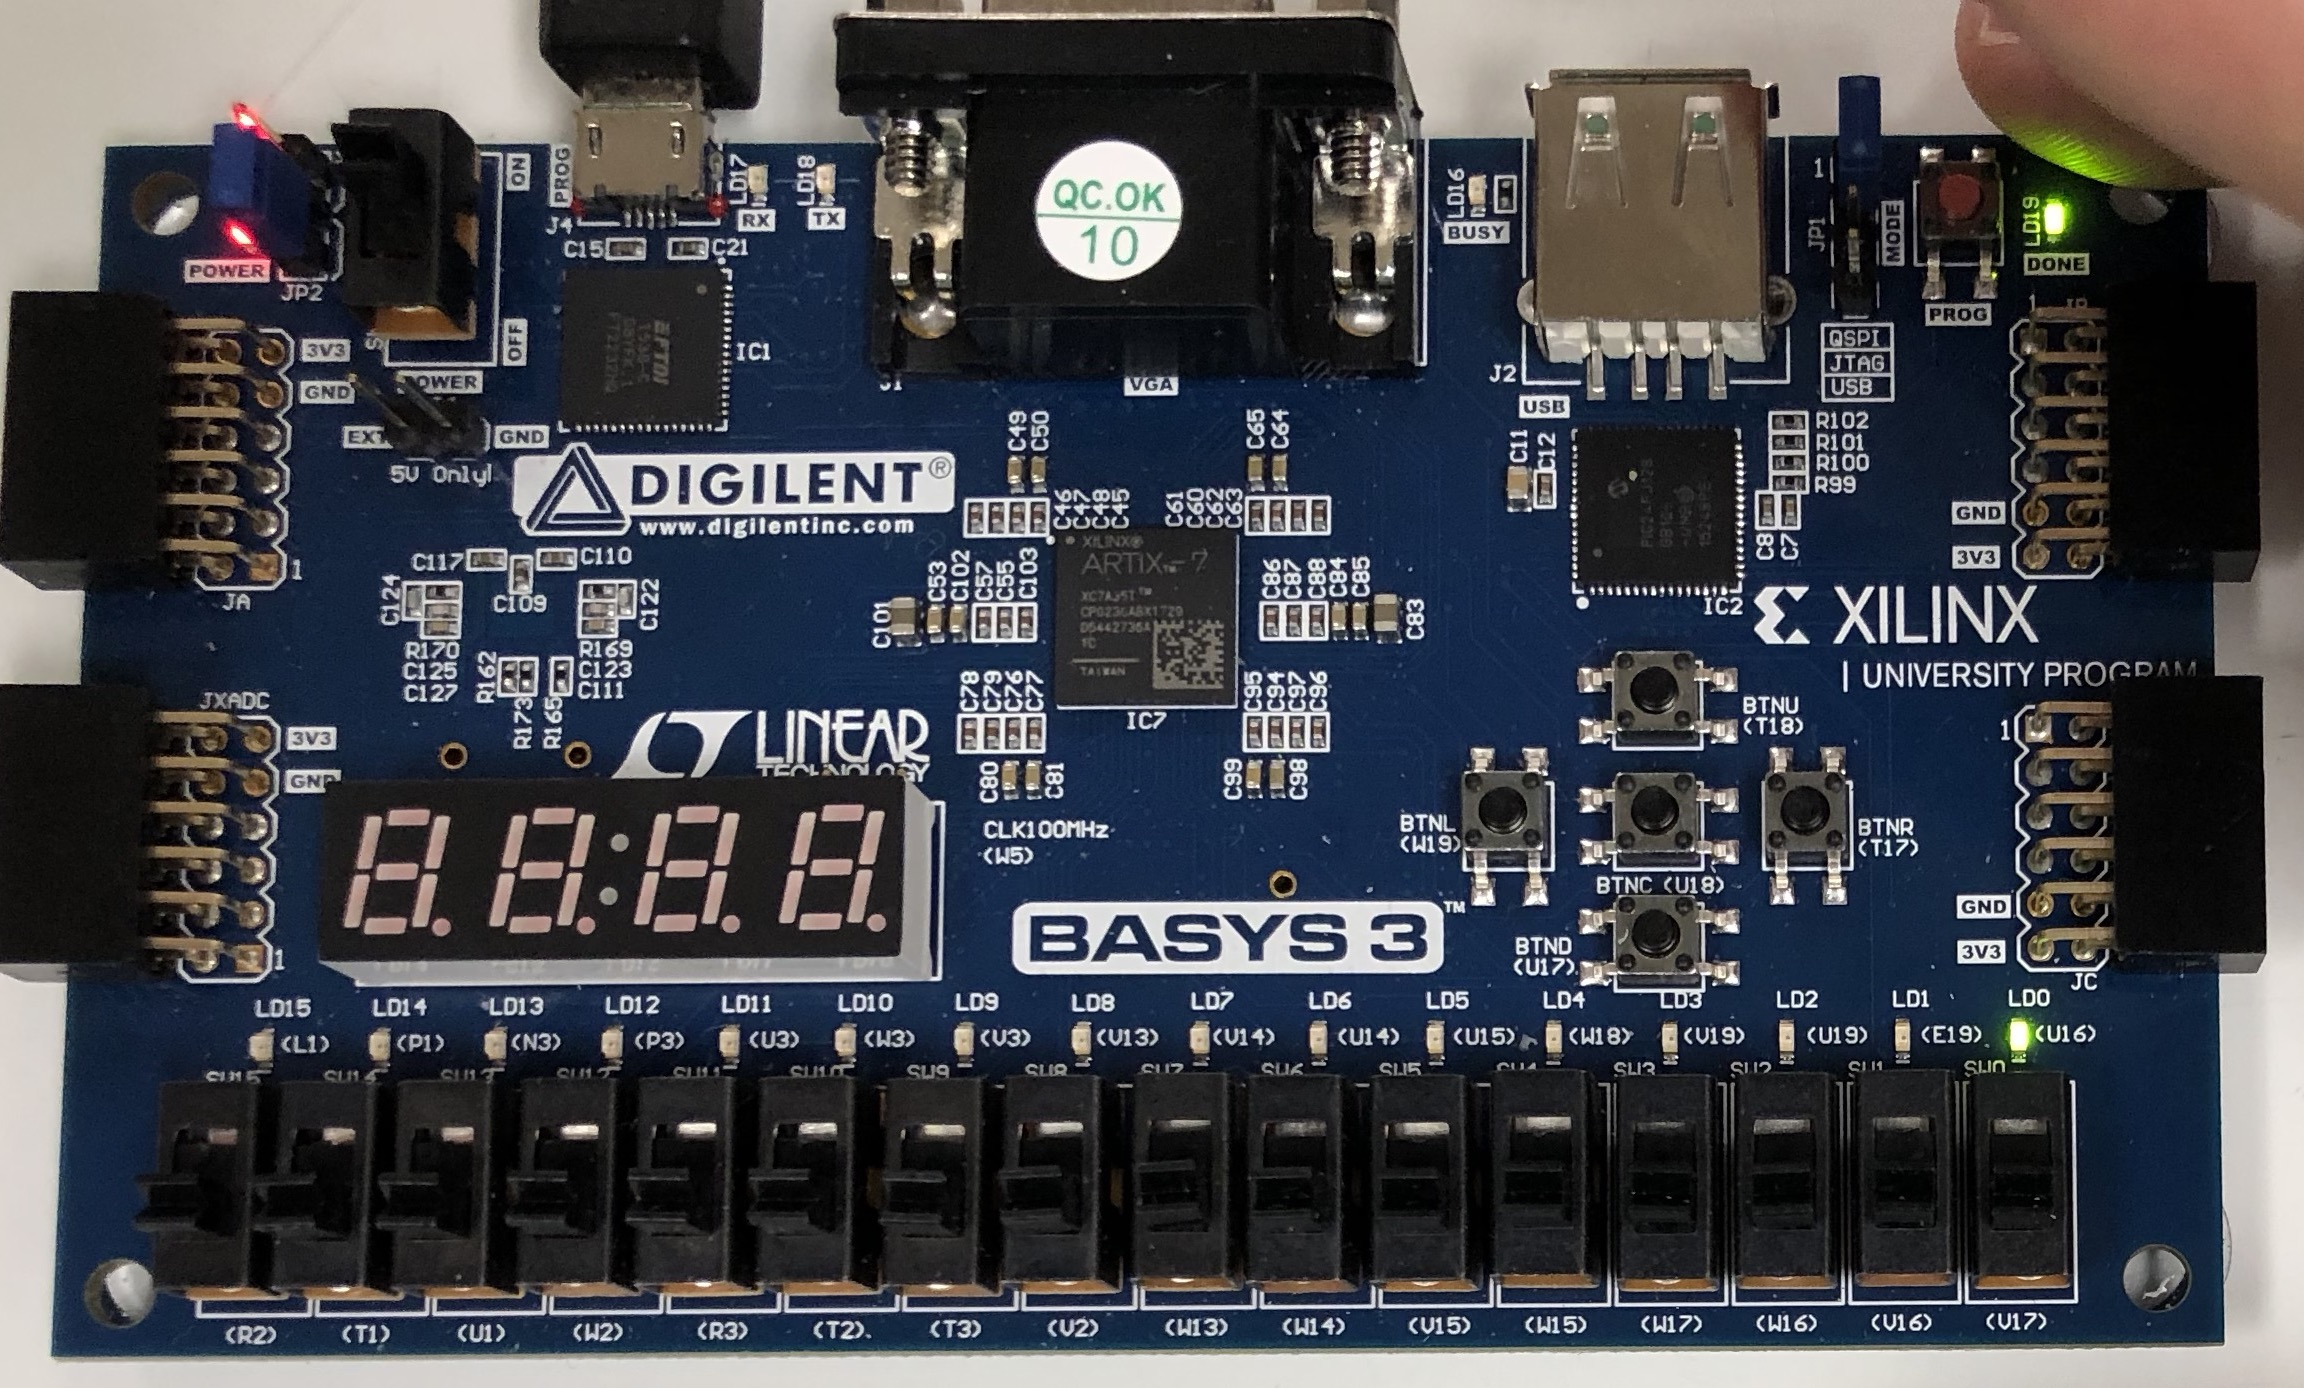
\includegraphics[width=0.5\textwidth]{./images/lab10img1.jpg}
	\caption{\label{fig:lab10_img1}No input, the amount is at 0.}
\end{center}
\end{figure}

\begin{figure}[H]
\begin{center}
	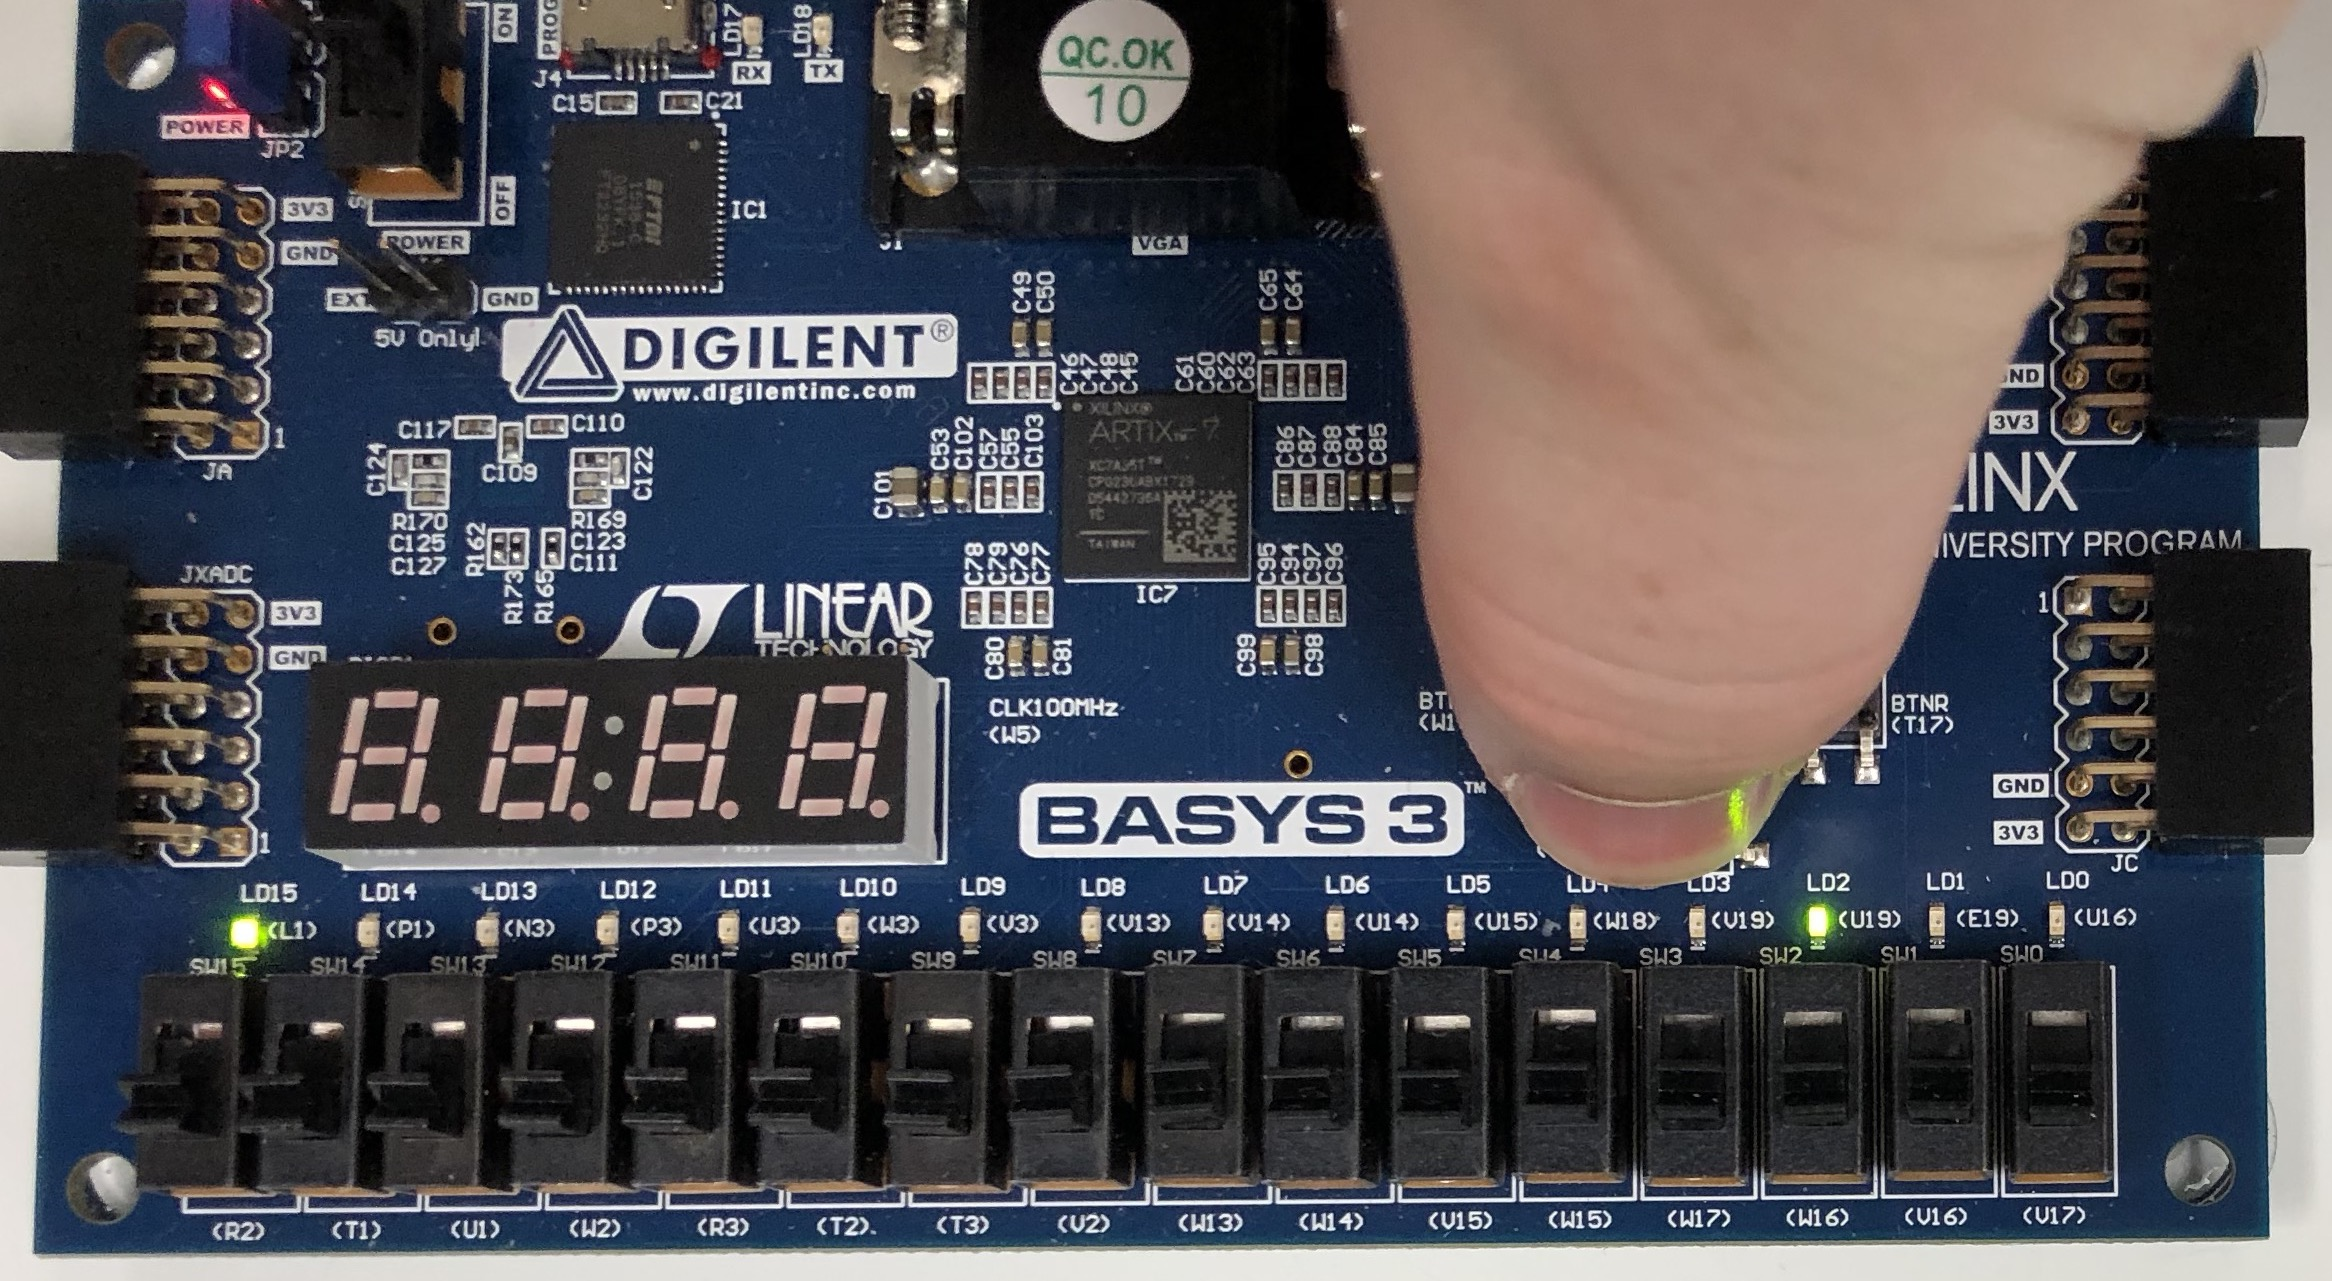
\includegraphics[width=0.5\textwidth]{./images/lab10img2.jpg}
	\caption{\label{fig:lab10_img2}One dime input, the amount is at 10 cents.}
\end{center}
\end{figure}

\begin{figure}[H]
\begin{center}
	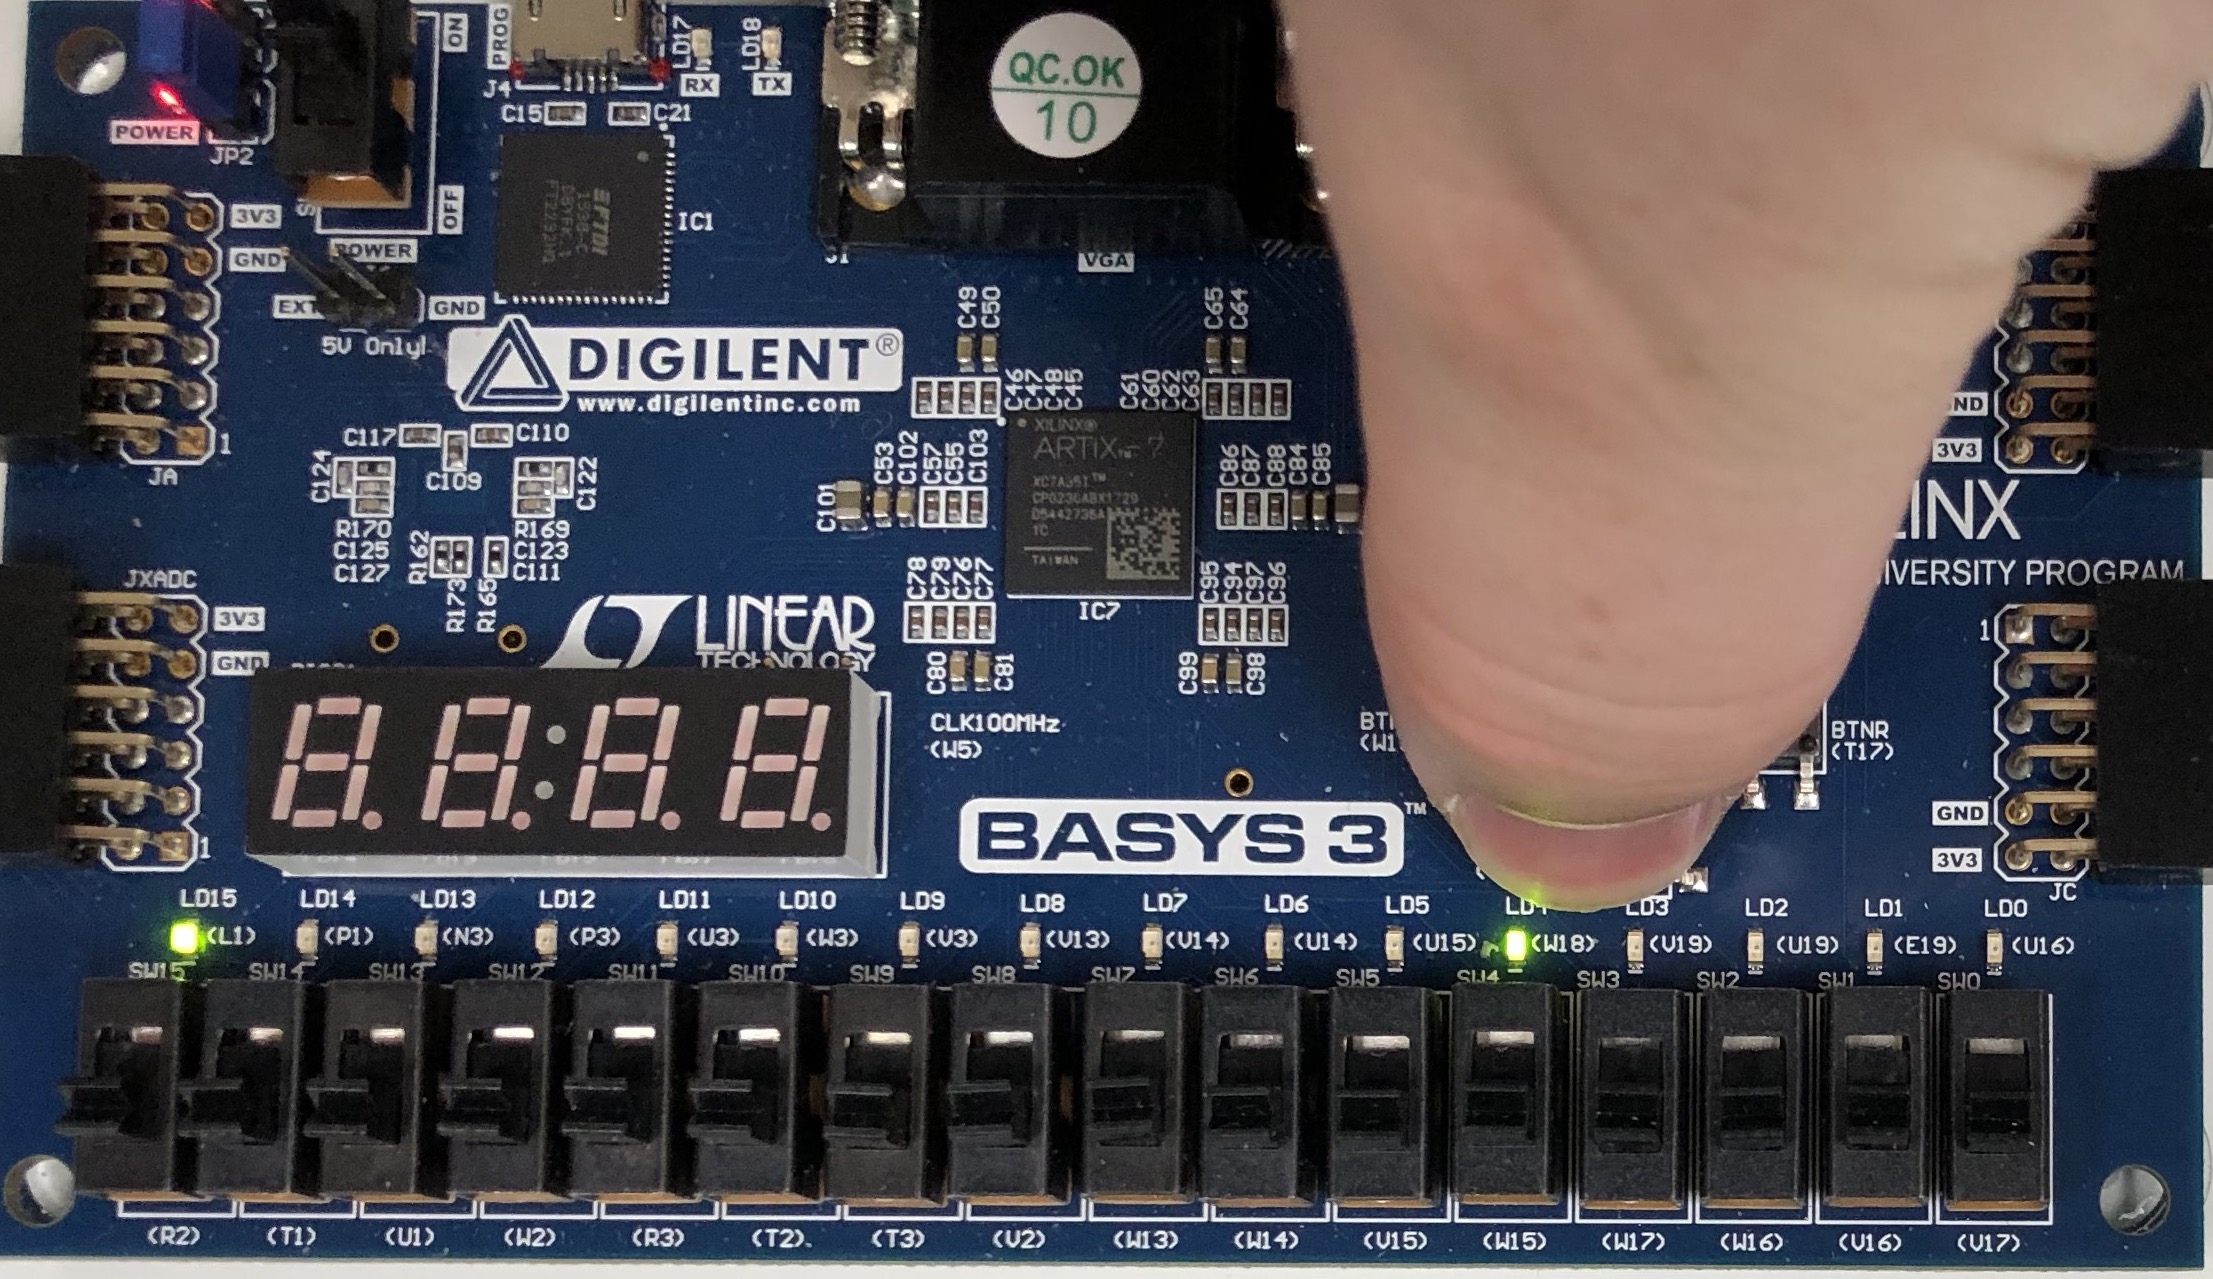
\includegraphics[width=0.5\textwidth]{./images/lab10img3.jpg}
	\caption{\label{fig:lab10_img3}Two dime inputs, the amount is at 20 cents, and no more coins are accepted.}
\end{center}
\end{figure}

\begin{figure}[H]
\begin{center}
	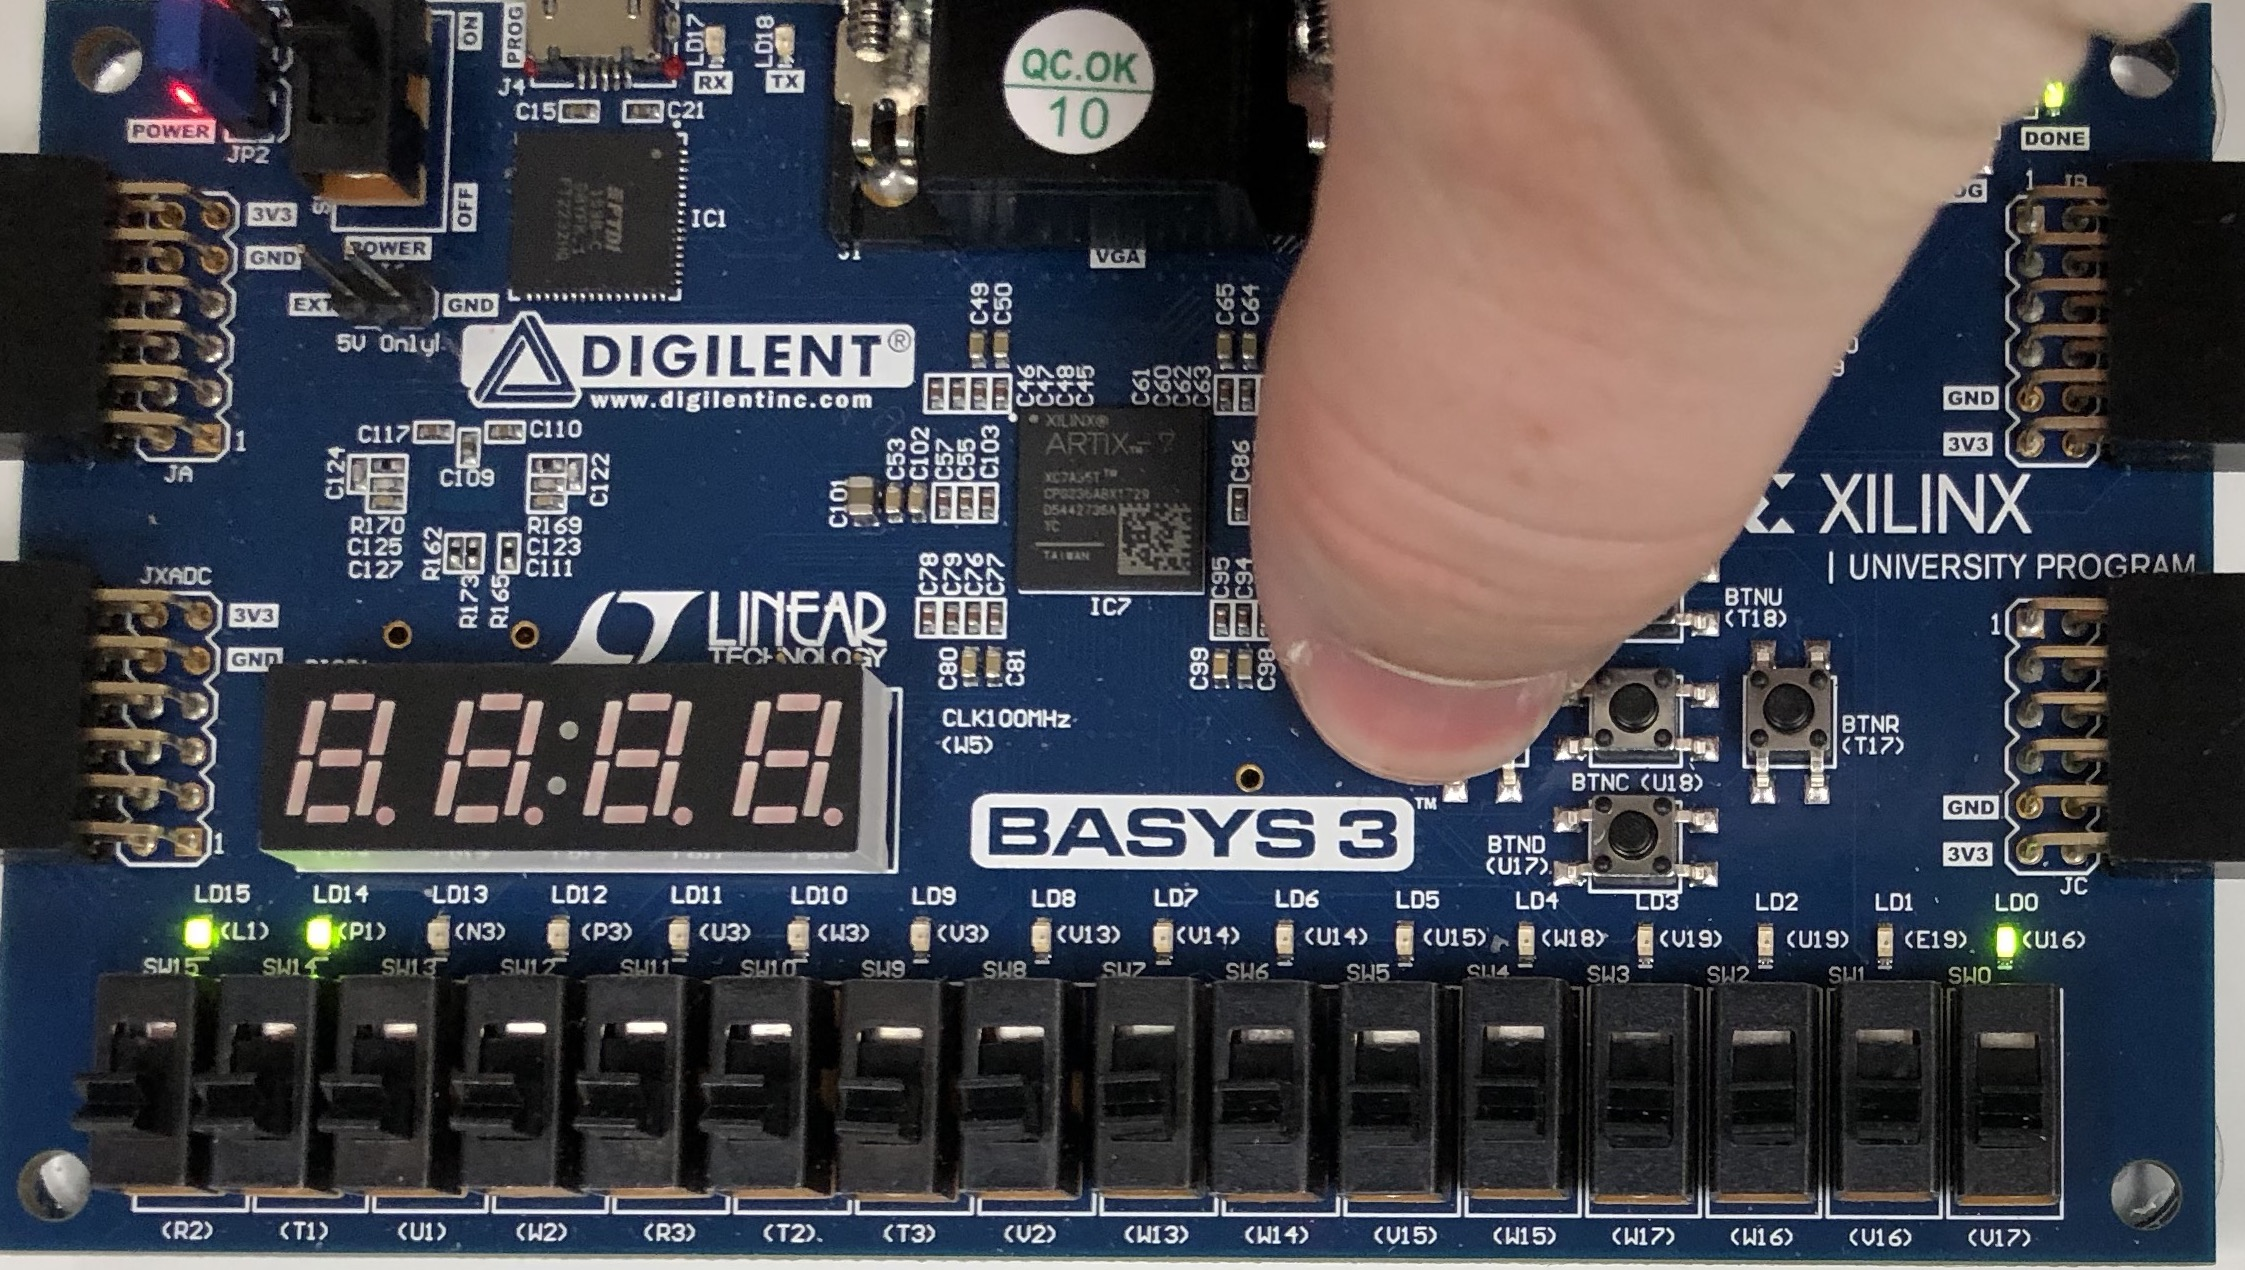
\includegraphics[width=0.5\textwidth]{./images/lab10img4.jpg}
	\caption{\label{fig:lab10_img4}Gum is selected, gum is being vended (as indicated by the LED on the left) and amount has returned to 0.}
\end{center}
\end{figure}

\begin{figure}[H]
\begin{center}
	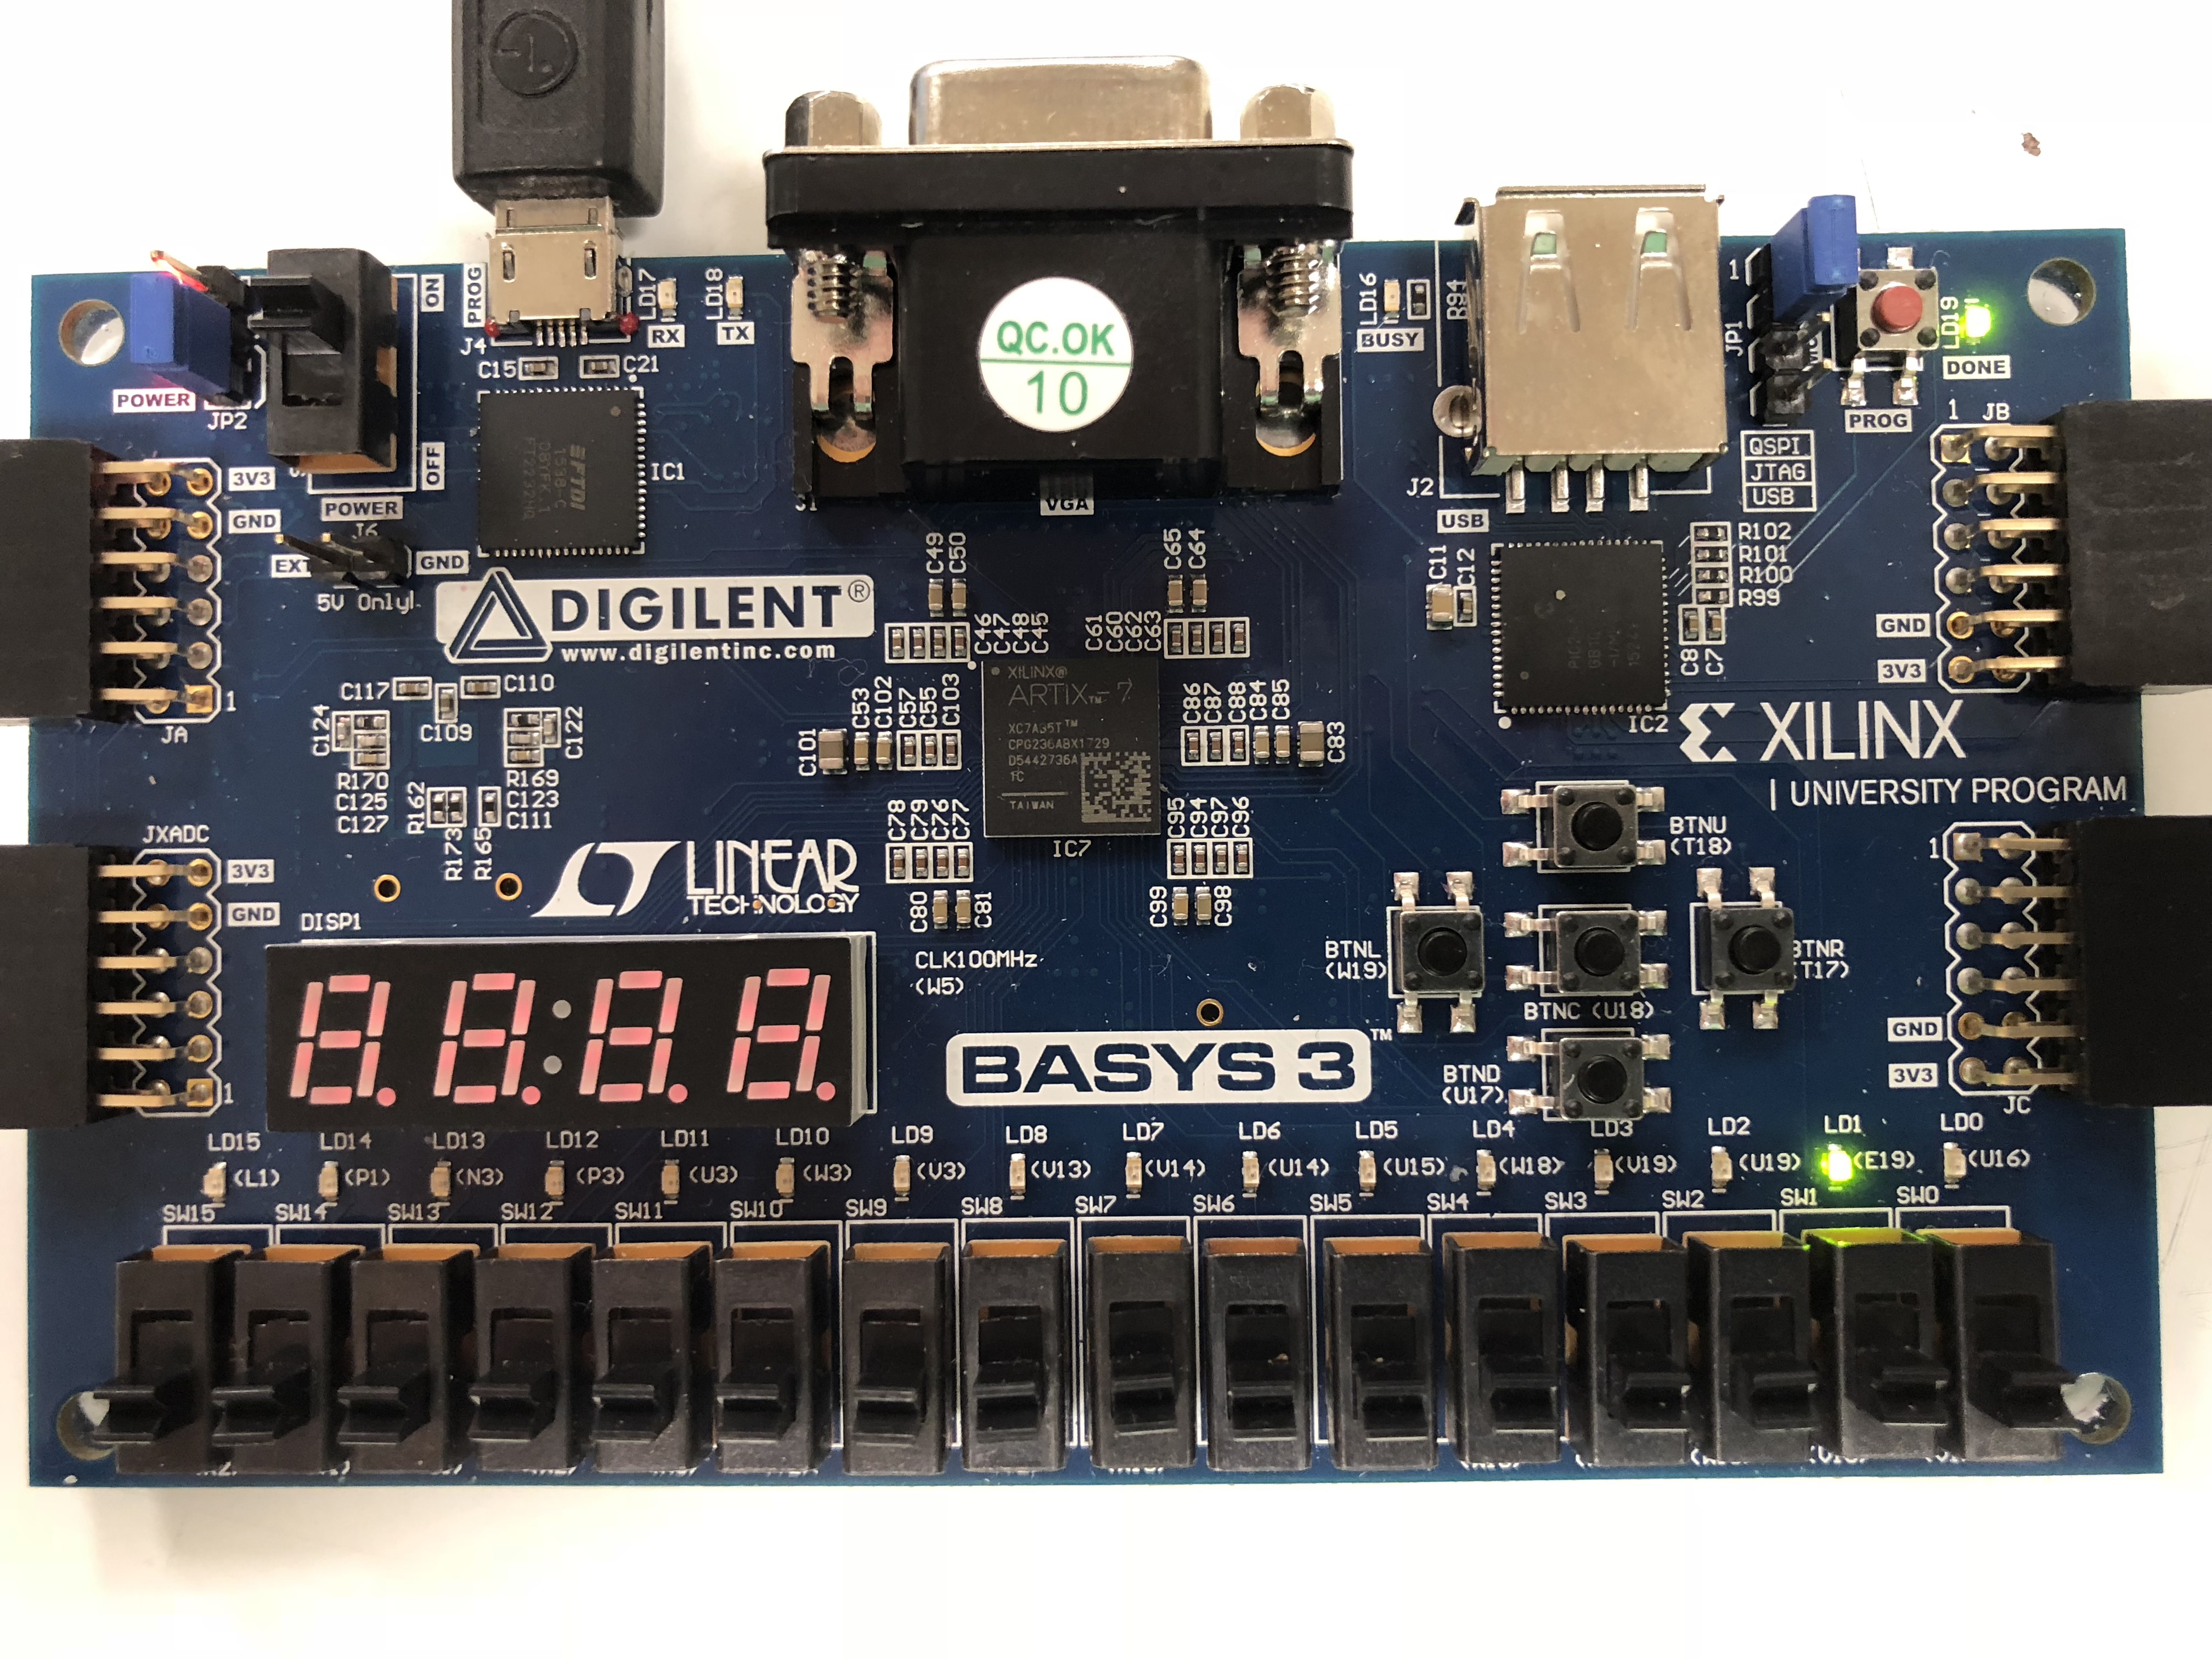
\includegraphics[width=0.5\textwidth]{./images/lab10img5.jpg}
	\caption{\label{fig:lab10_img5}One nickel inserted, amount is at 5 cents.}
\end{center}
\end{figure}

\begin{figure}[H]
\begin{center}
	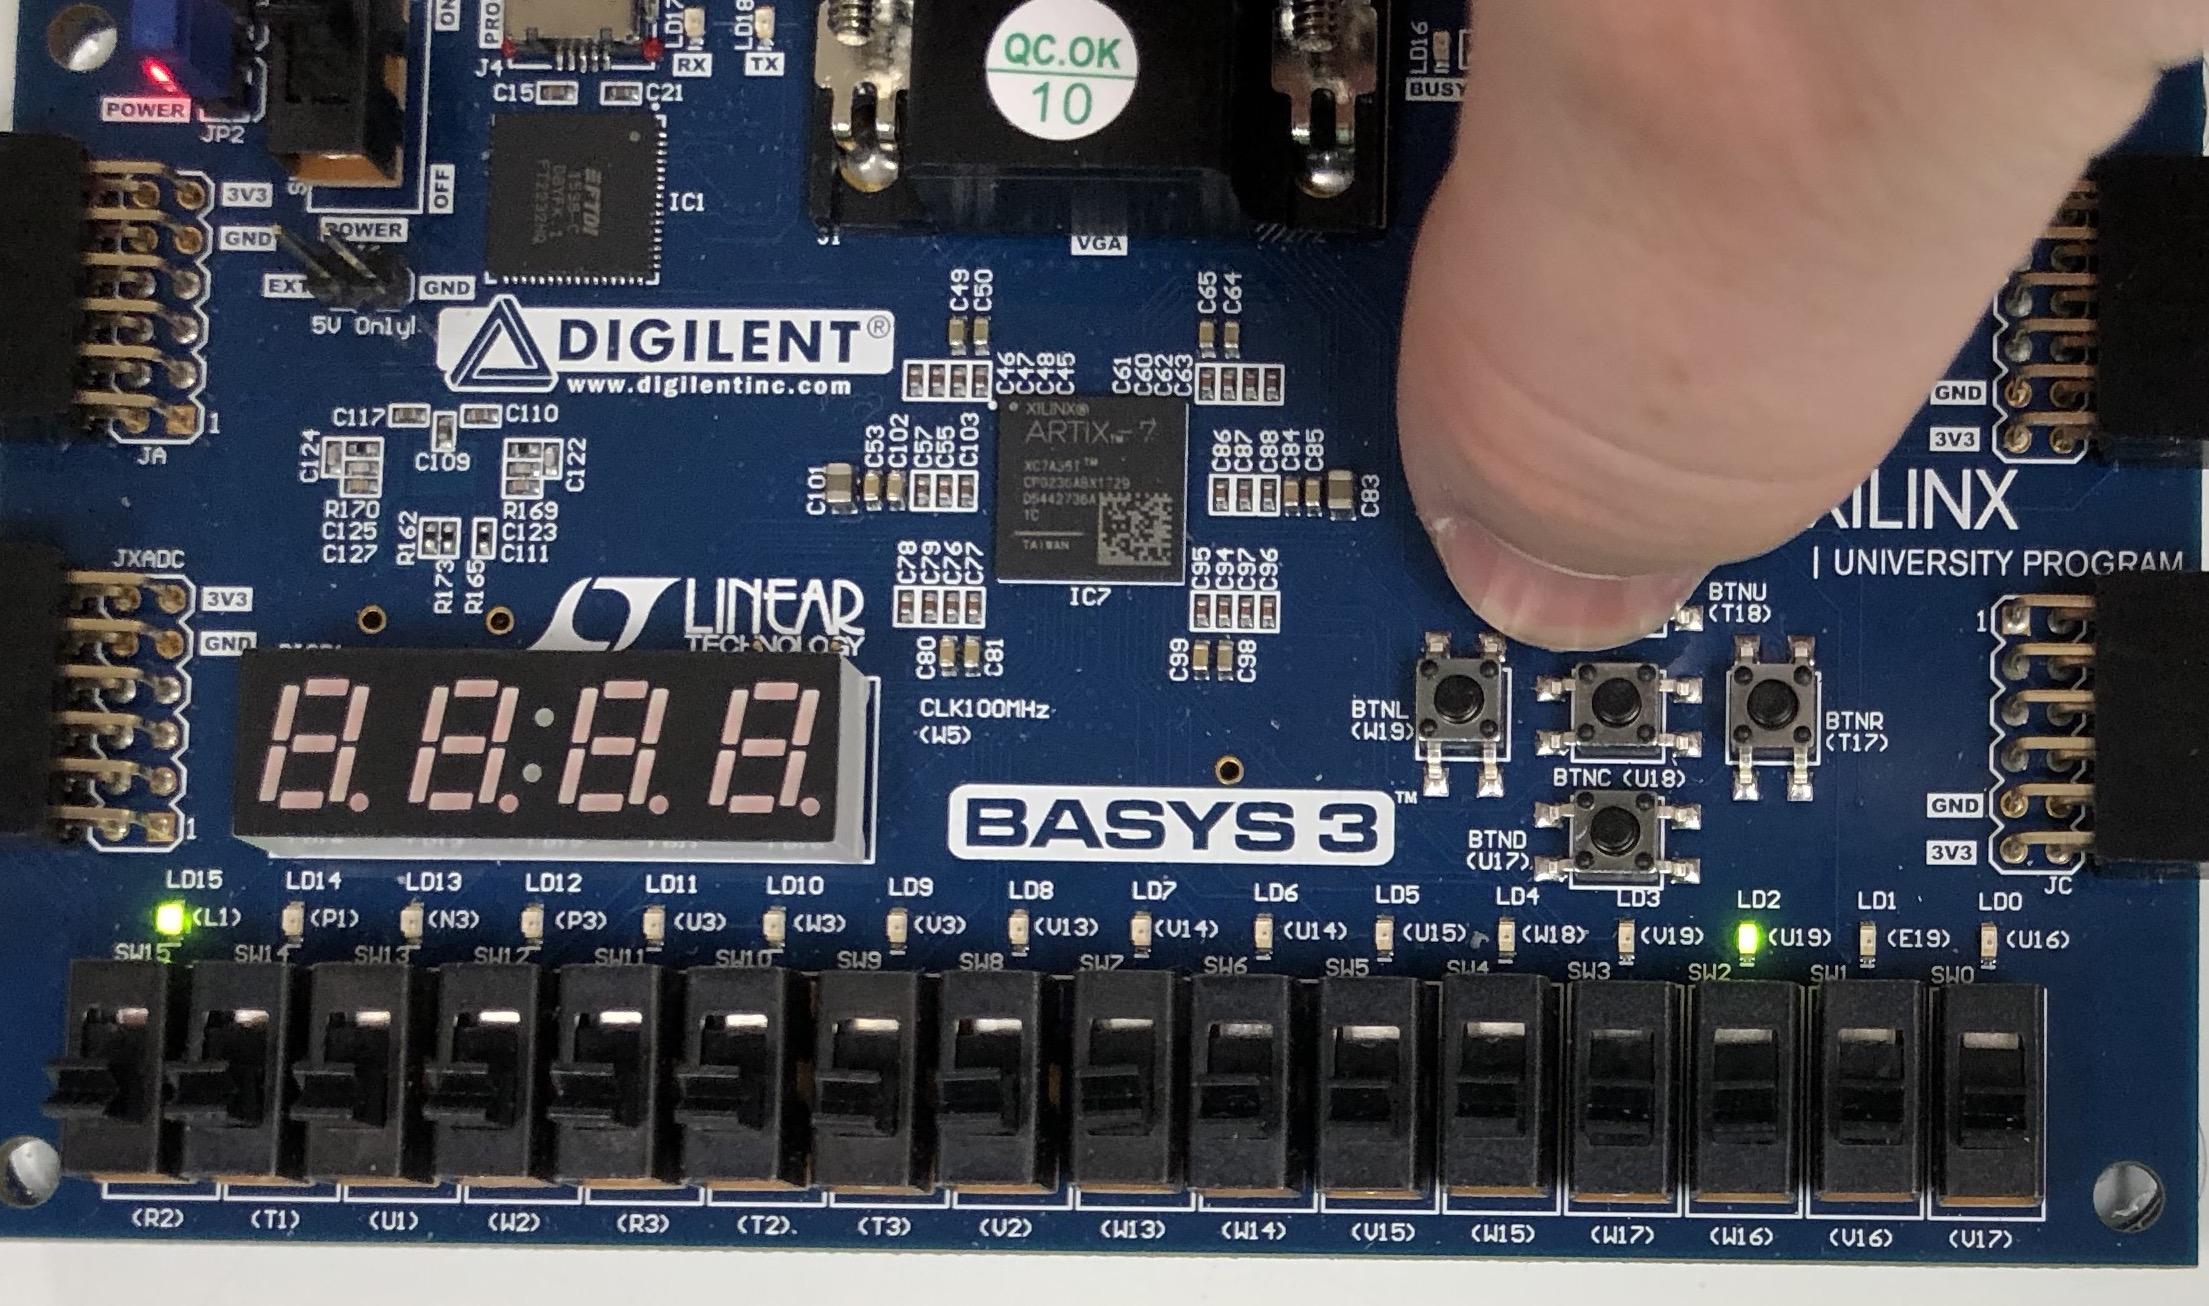
\includegraphics[width=0.5\textwidth]{./images/lab10img6.jpg}
	\caption{\label{fig:lab10_img6}Two nickels are inserted, amount is at 10 cents.}
\end{center}
\end{figure}

\begin{figure}[H]
\begin{center}
	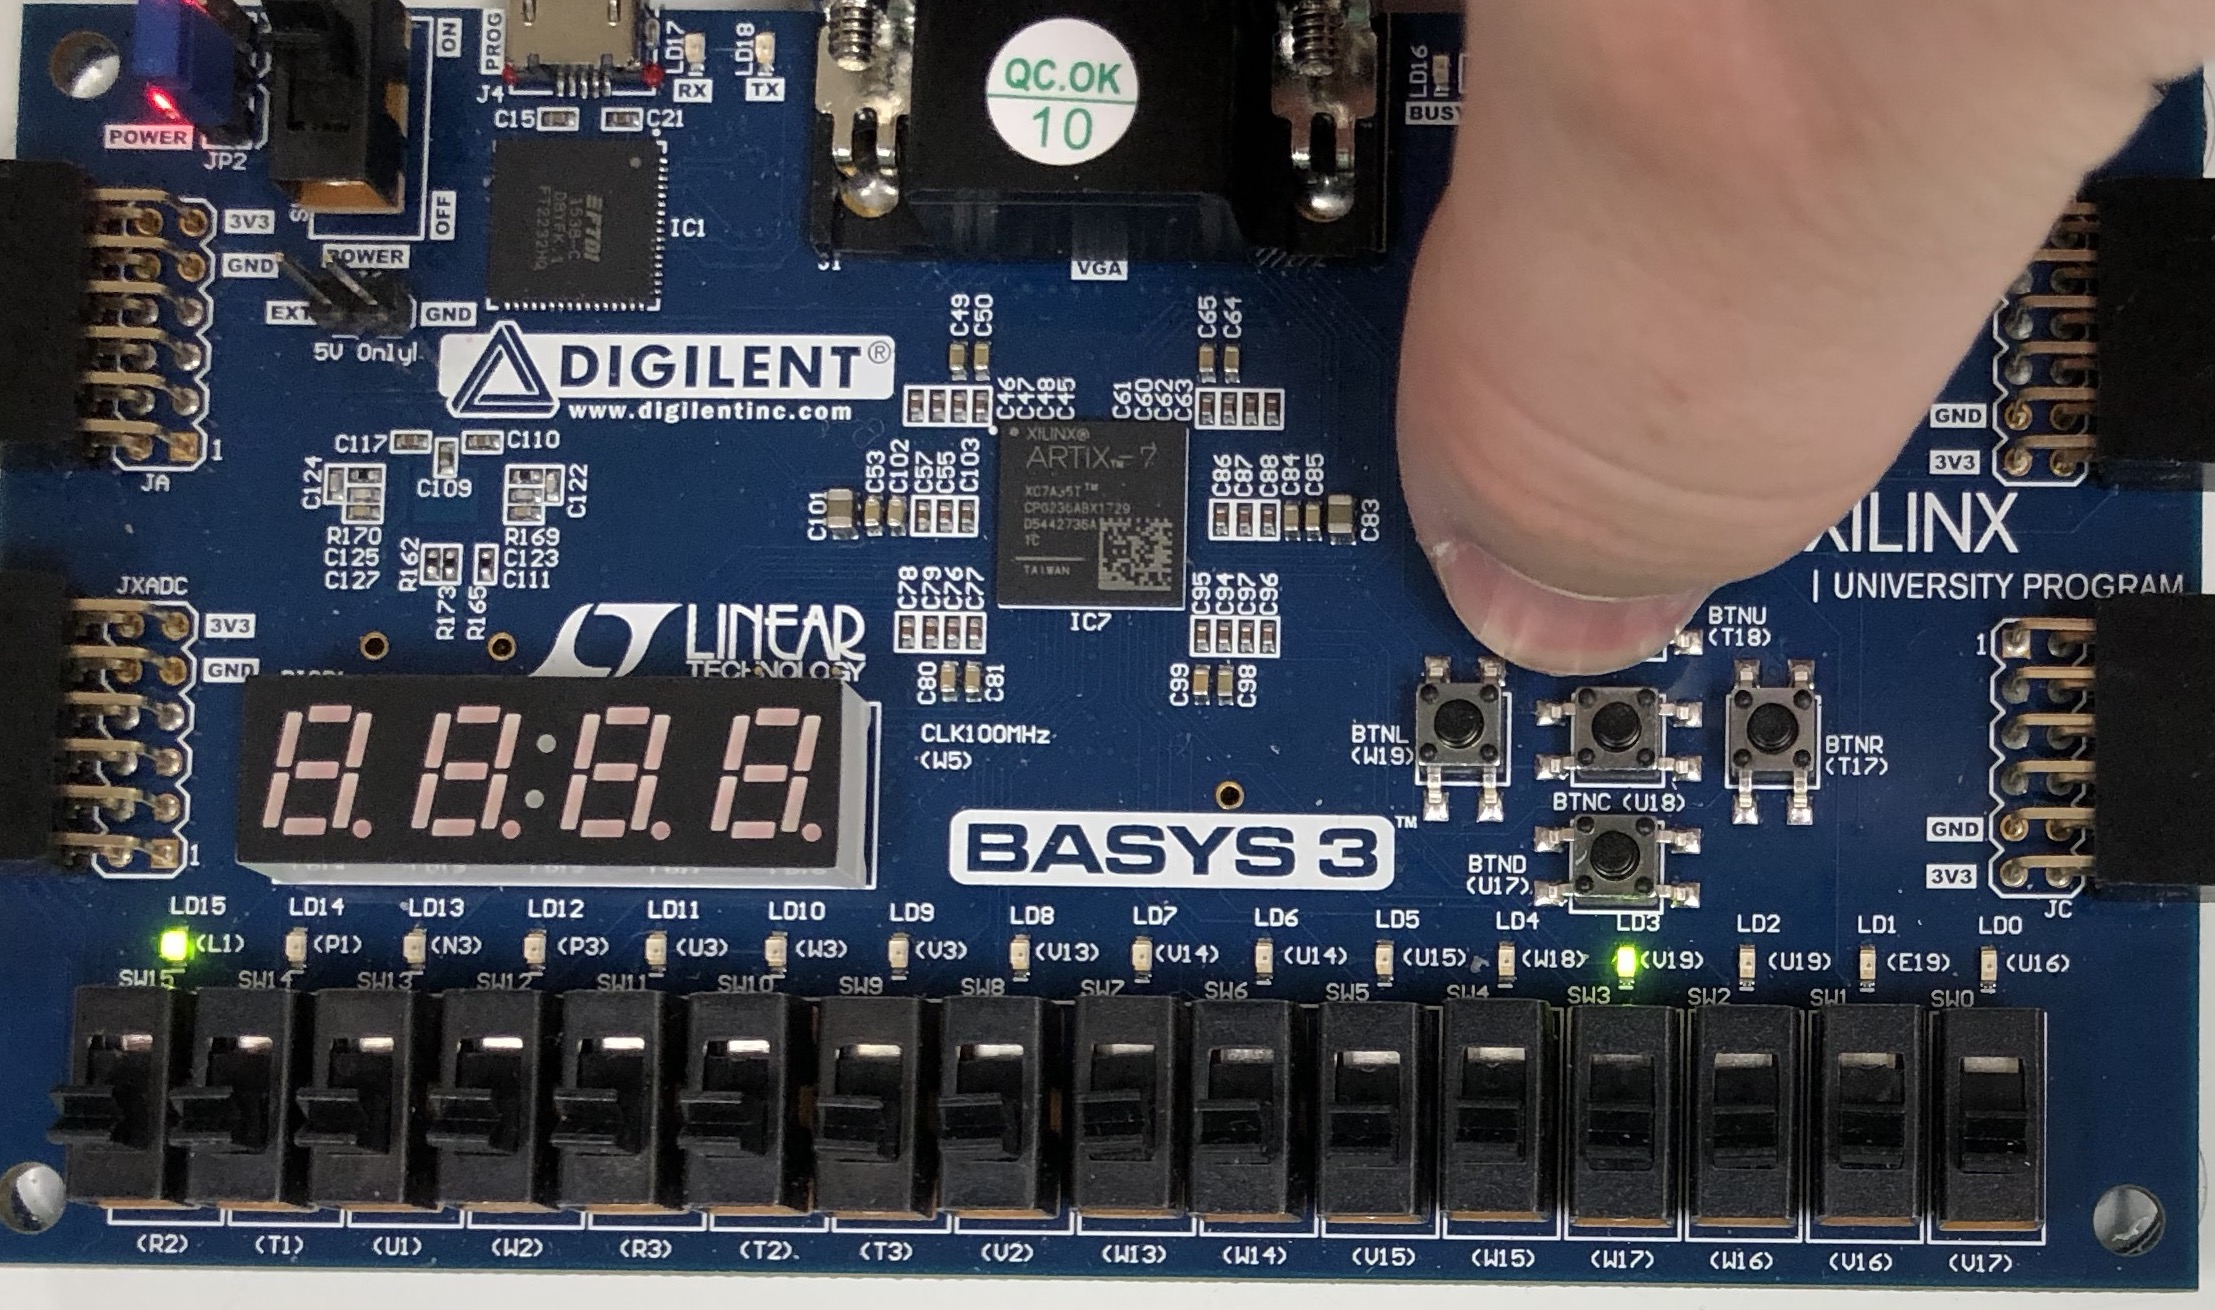
\includegraphics[width=0.5\textwidth]{./images/lab10img7.jpg}
	\caption{\label{fig:lab10_img7}Three nickels are inserted, amount is at 15 cents.}
\end{center}
\end{figure}

\begin{figure}[H]
\begin{center}
	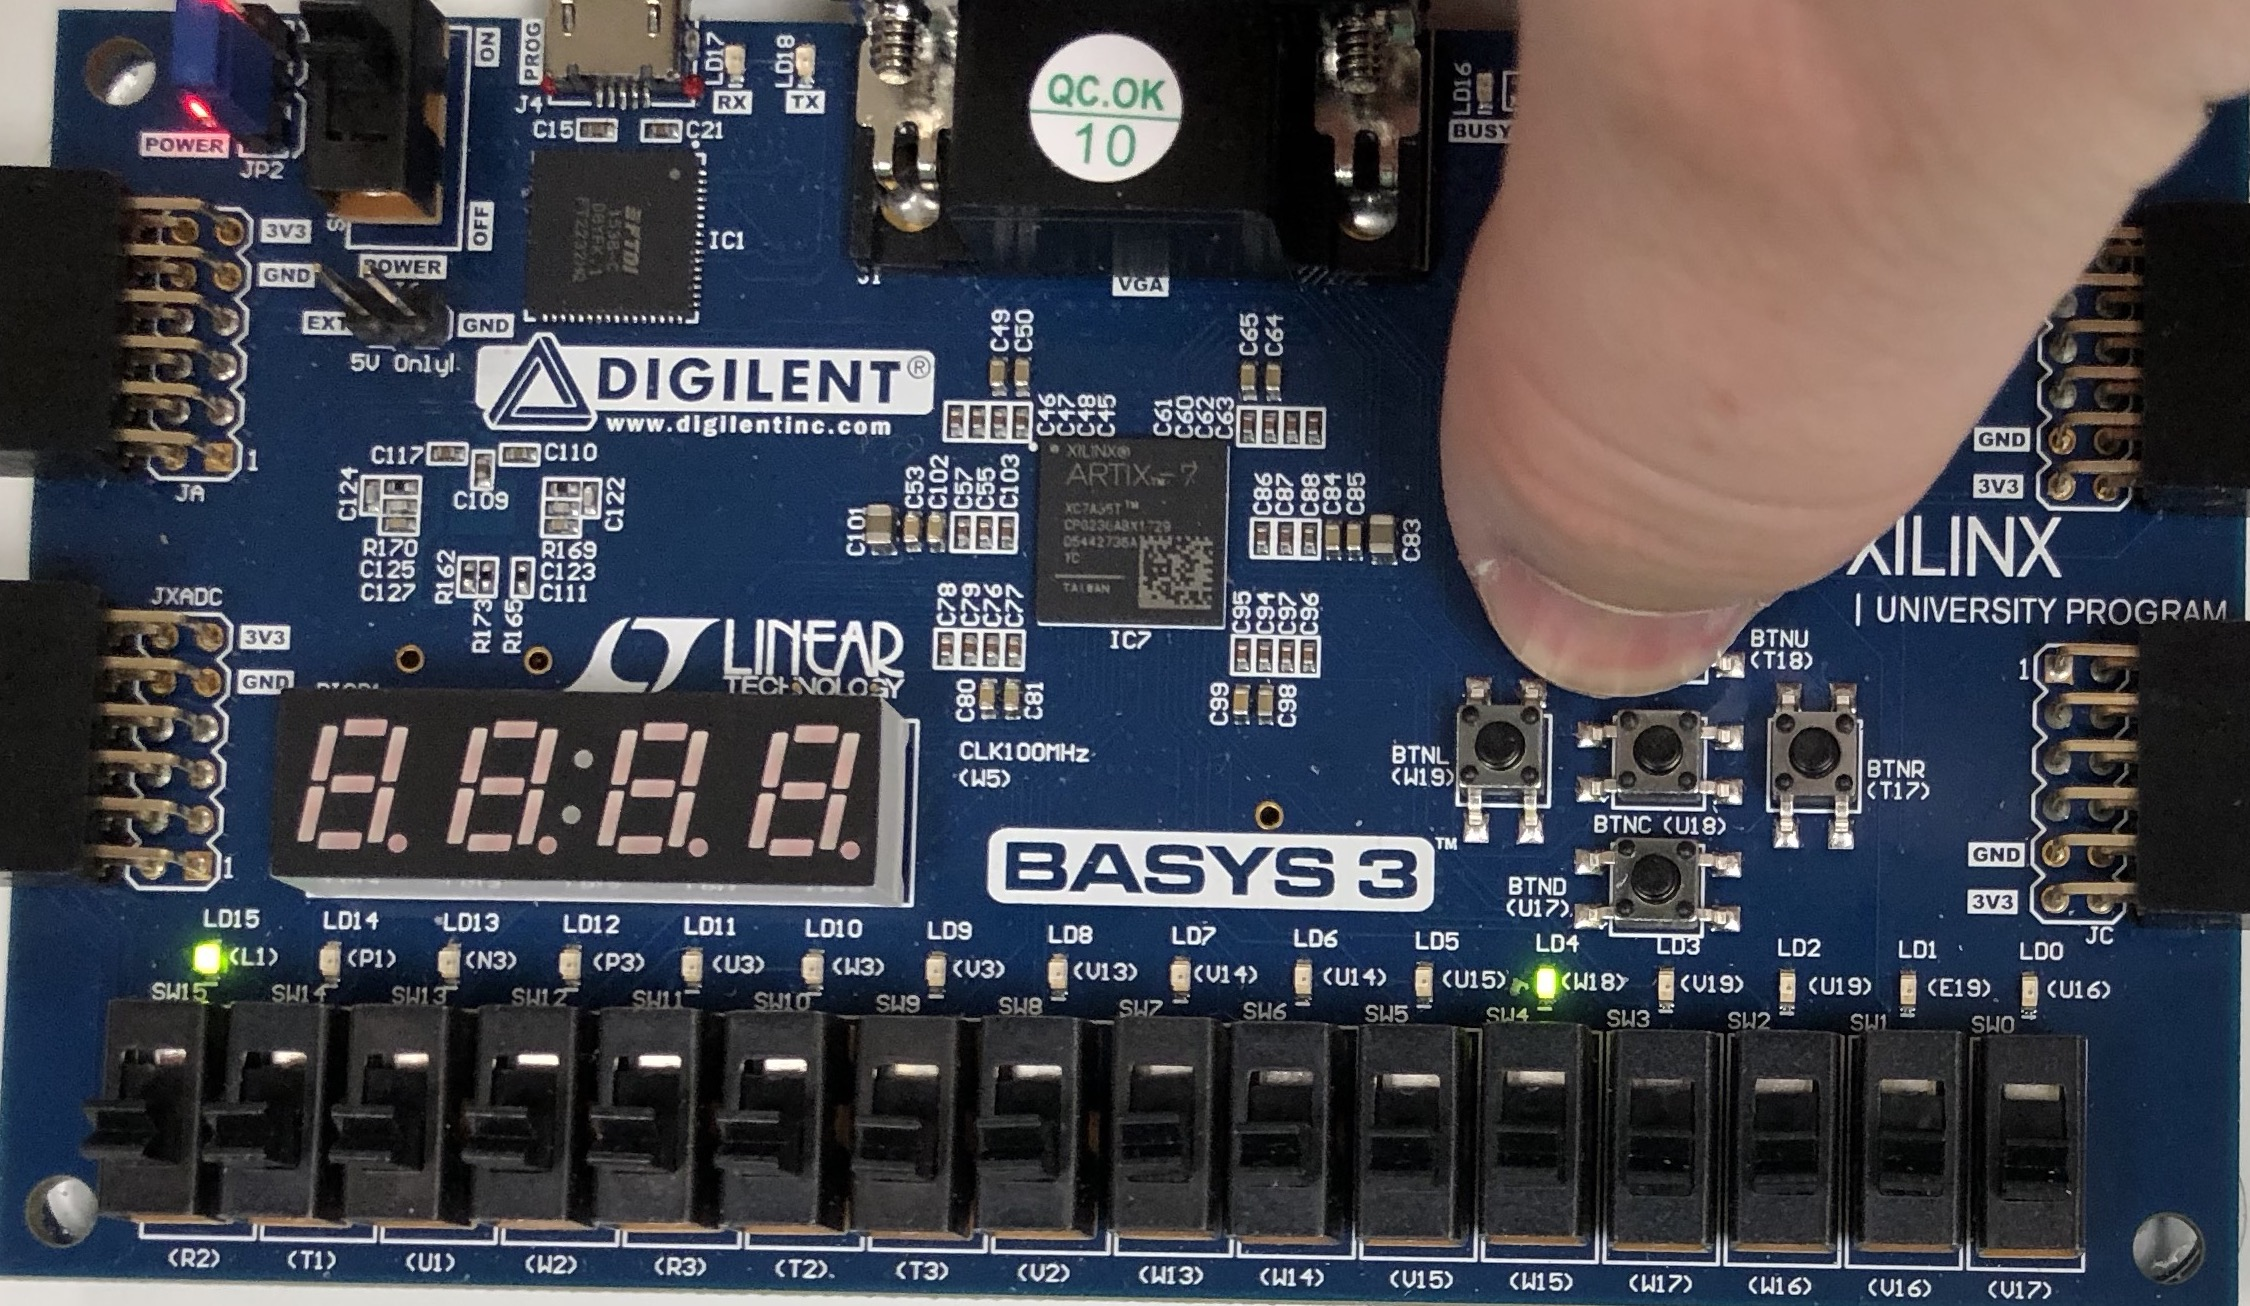
\includegraphics[width=0.5\textwidth]{./images/lab10img8.jpg}
	\caption{\label{fig:lab10_img8}Four nickels are inserted, amount is at 20 cents.}
\end{center}
\end{figure}

\begin{figure}[H]
\begin{center}
	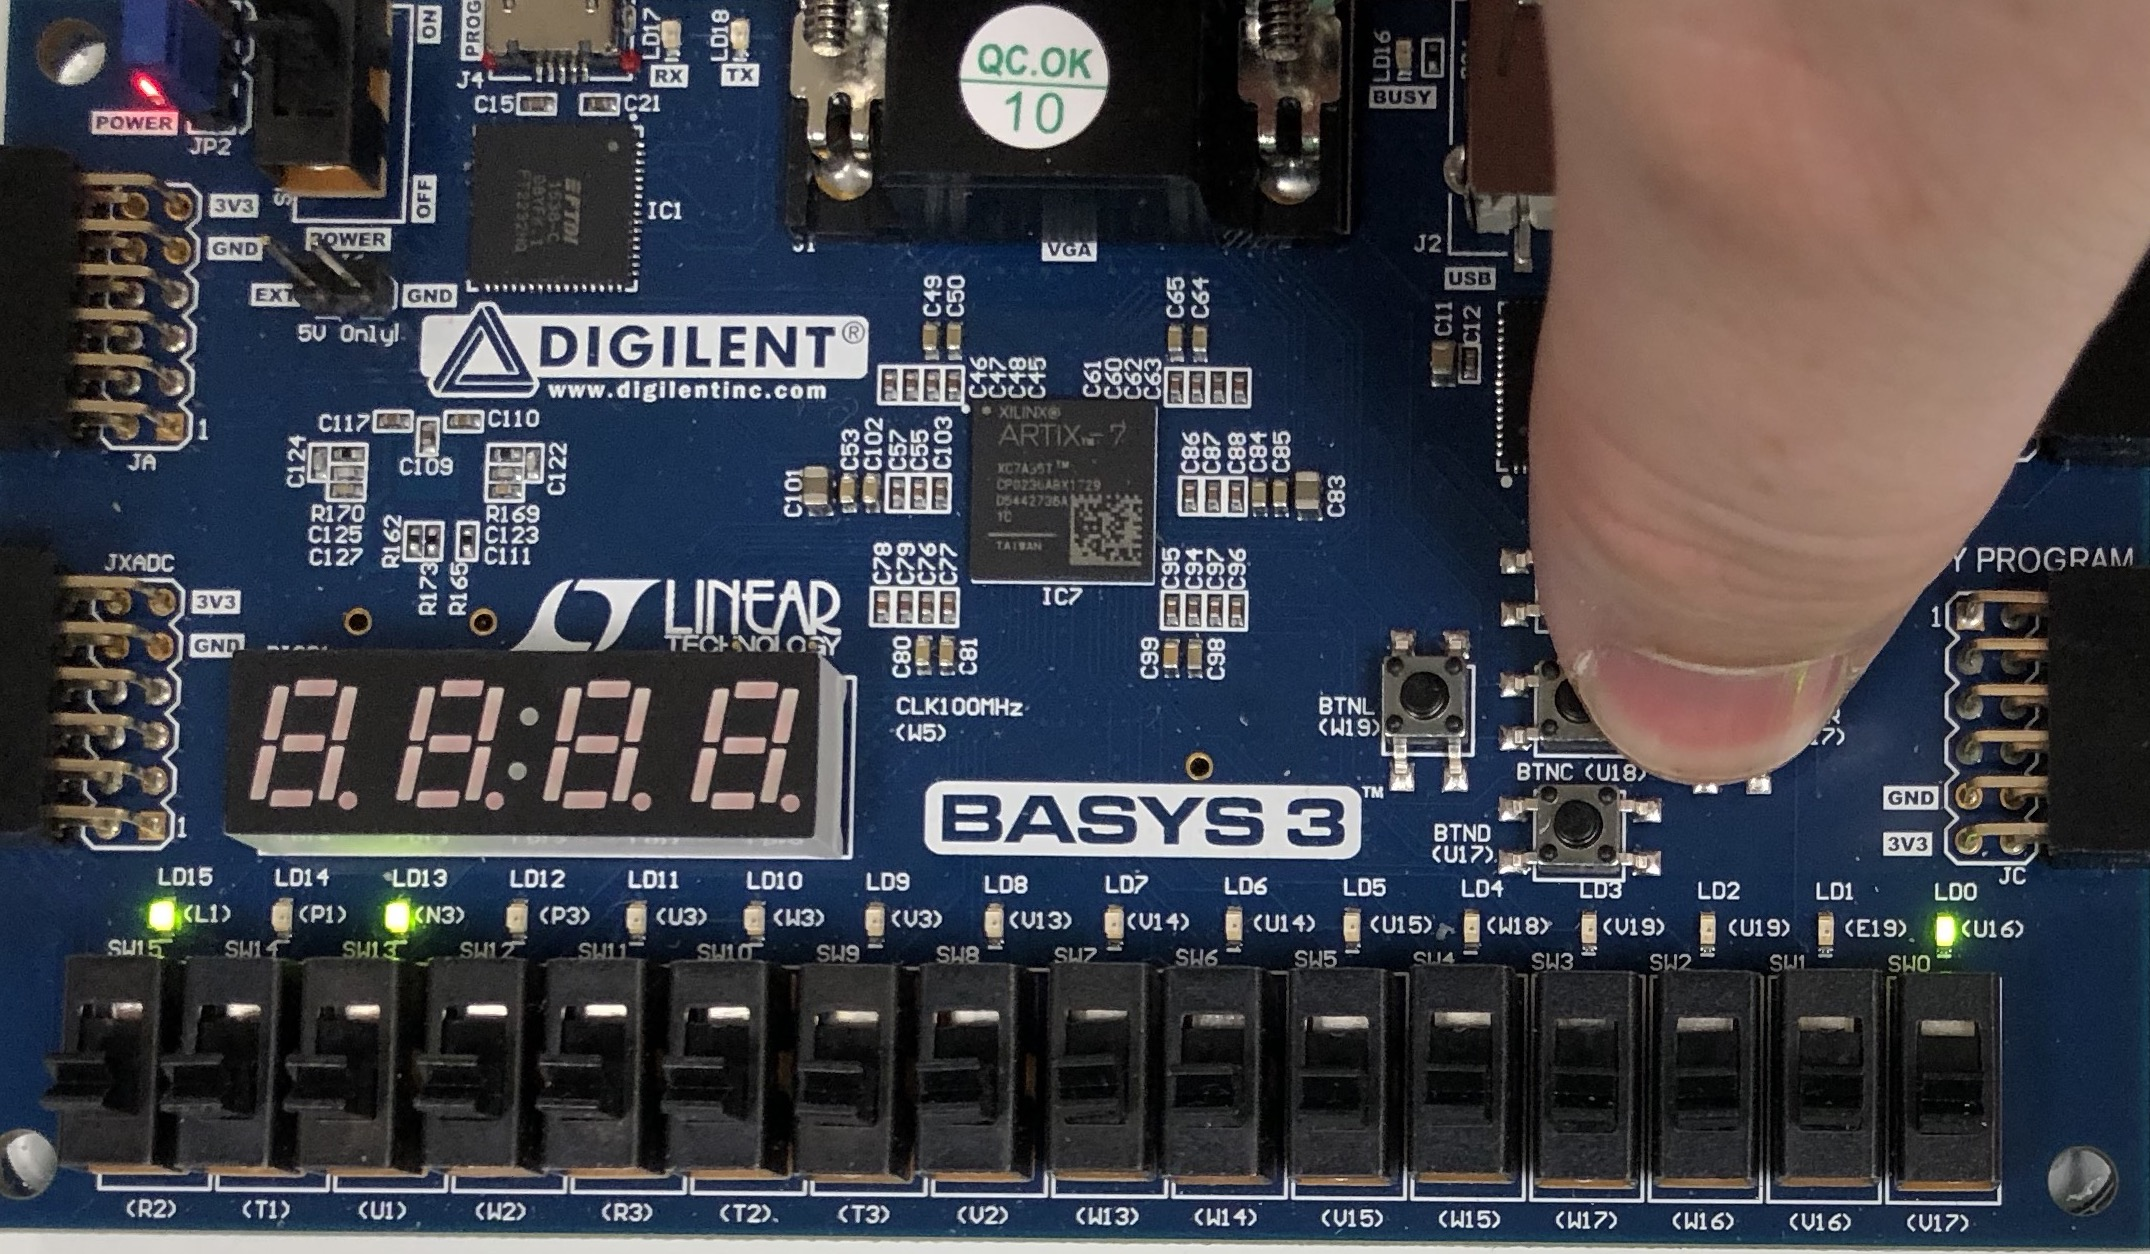
\includegraphics[width=0.5\textwidth]{./images/lab10img9.jpg}
	\caption{\label{fig:lab10_img9}Candy is selected, and is vending (as shown by LED on left). Amount returns to 0.}
\end{center}
\end{figure}

\section{Conclusion}
In this lab we successfully implemented the vending machine. The most difficult technical challenge was developing the state diagram in the prelab. Once we had our diagram completed, we found it relatively simple to implement on the board.

\pagebreak

\textbf{Appendices}

\begin{appendices}

\section{Clock Divider VHDL Code}
This code for a clock divider is used in the lab.

\begin{lstlisting}[language=VHDL]
library IEEE;
use IEEE.STD_LOGIC_1164.ALL;
use IEEE.NUMERIC_STD.ALL;

entity Clockdivider is
     port(clk : in std_logic;
          start_timer : in std_logic;
	  FastClock,MediumClock,SlowClock, led0 : out std_logic);
end Clockdivider;

architecture clockdivider_arch of Clockdivider is
signal slowClock_sig : STD_LOGIC;
begin
    process  
    variable cnt :	std_logic_vector(26 downto 0):=
     "000000000000000000000000000";
    begin					 
        wait until ((clk'EVENT) AND (clk = '1'));
		if (start_timer = '1') then
	       cnt := "000000000000000000000000000";
	    else  
           cnt := STD_LOGIC_VECTOR(unsigned(cnt) + 1);
	    end if;
   	    FastClock <= cnt(22);
   	    MediumClock <= cnt(24);	
   	    SlowClock <= cnt(26);
        slowClock_sig <= cnt(26);
        if (slowClock_sig = '1') then
		  led0 <= '1';
	    else
		  led0 <= '0';
	    end if;
	end process;
end clockdivider_arch;
\end{lstlisting}

\section{Problem 1 VHDL Code}

\begin{lstlisting}[language=VHDL]
library IEEE;
use IEEE.STD_LOGIC_1164.ALL;

entity vending_machine is
    Port ( clk, reset, nickel, dime, gum, candy : in STD_LOGIC;
    amount : out STD_LOGIC_VECTOR(4 downto 0);
    dispense_gum, dispense_candy, clock_led : out STD_LOGIC);
end vending_machine;

architecture Behavioral of vending_machine is

component clock_divider is
     port(clk : in std_logic;
          start_timer : in std_logic;
	  FastClock,MediumClock,SlowClock, led0 : out std_logic);
end component clock_divider;

signal current_state : STD_LOGIC_VECTOR(2 downto 0) := "000";
signal next_state : STD_LOGIC_VECTOR(2 downto 0) := "000";
signal reset_clock : STD_LOGIC := '0';
signal fast_clock, medium_clock, slow_clock : STD_LOGIC;

begin

    cd : clock_divider port map(clk, reset_clock, fast_clock, 
    		medium_clock, slow_clock, clock_led);

    process(slow_clock, reset)
    begin
        if(reset = '1') then next_state <= "000";
        elsif(slow_clock'event and slow_clock = '1') then
            case current_state is
                when "000" =>
                    if(dime = '1') then next_state <= "010";
                    elsif(nickel = '1') then next_state <= "001";
                    else next_state <= "000";
                    end if;
                when "001" =>
                    if(dime = '1') then next_state <= "011";
                    elsif(nickel = '1') then next_state <= "010";
                    else next_state <= "001";
                    end if;
                when "010" =>
                    if(dime = '1') then next_state <= "100";
                    elsif(nickel = '1') then next_state <= "011";
                    else next_state <= "010";
                    end if;
                when "011" =>
                    if(dime = '1' or nickel = '1') then next_state <= "100";
                    elsif(gum = '1') then next_state <= "101";
                    else next_state <= "011";
                    end if;
                when "100" =>
                    if(candy = '1') then next_state <= "110";
                    elsif(gum = '1') then next_state <= "101";
                    else next_state <= "100";
                    end if;
                when others =>
                    next_state <= "000";
            end case;
        end if;
    end process;
    process(current_state)
    begin
        case current_state is
            when "000" =>
                amount <= "00001";
                dispense_gum <= '0';
                dispense_candy <= '0';
            when "001" =>
                amount <= "00010";
                dispense_gum <= '0';
                dispense_candy <= '0';
            when "010" =>
                amount <= "00100";
                dispense_gum <= '0';
                dispense_candy <= '0';
            when "011" =>
                amount <= "01000";
                dispense_gum <= '0';
                dispense_candy <= '0';
            when "100" =>
                amount <= "10000";
                dispense_gum <= '0';
                dispense_candy <= '0';
            when "101" =>
                amount <= "00001";
                dispense_gum <= '1';
                dispense_candy <= '0';
            when "110" =>
                amount <= "00001";
                dispense_gum <= '0';
                dispense_candy <= '1';
            when others =>
                amount <= "00001";
                dispense_gum <= '0';
                dispense_candy <= '0';
        end case;
    end process;
    current_state <= next_state;

end Behavioral;
\end{lstlisting}

\section{Problem 1 Constraints File}
\begin{center}
\begin{figure}[H]
	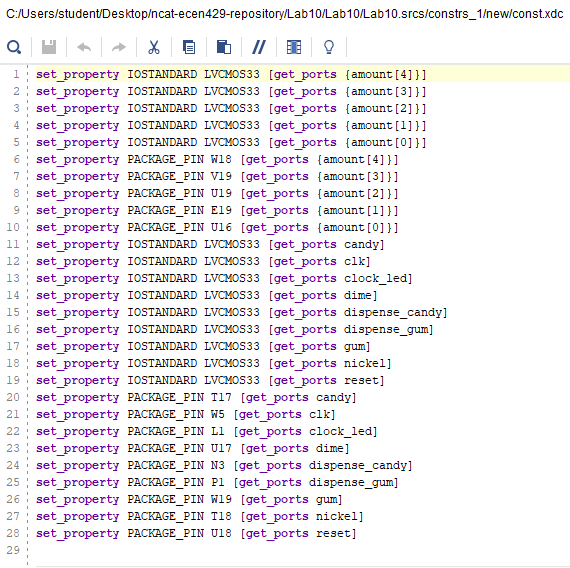
\includegraphics[scale=1]{./images/const.png}
	\caption{\label{fig:Prob1Const}Constraints file for Lab 10.}
\end{figure}
\end{center}

\end{appendices}
\end{document}
